\section{Introduction}

To solve a problem using Reinforcement Learning (RL), it is necessary first to formalise that problem using a reward function \citep{sutton2018}. 
However, due to the complexity of many real-world tasks, it is exceedingly difficult to directly specify a reward function that fully captures the task in the intended way.
However, misspecified reward functions will often lead to undesirable behaviour \citep{paulus2017deep, ibarz2018reward, knox2022reward, reward_misspecification}. This makes designing good reward functions a major obstacle to using RL in practice, especially for safety-critical applications.

An increasingly popular solution is to \emph{learn} reward functions from mechanisms such as human or automated feedback \cite[e.g.\ ][]{NIPS2017_d5e2c0ad, ng2000}.
However, this approach comes with its own set of challenges: 
the right data can be difficult to collect \cite[e.g.\ ][]{paulus2017deep}, and it is often challenging to interpret it correctly \cite[e.g.\ ][]{armstrong2019occams, skalse2023misspecification}.
Moreover, optimising a policy against a learned reward model effectively constitutes a distributional shift \citep{gao_scaling_2022}; i.e., even if a reward function is accurate under the training distribution, it may fail to induce desirable behaviour from the RL agent.

Therefore in practice it is often more appropriate to think of the reward function as a \emph{proxy} for the true objective rather than \emph{being} the true objective. %, and it should not be assumed to always be accurate.
This means that we need a more principled and comprehensive understanding of what happens when a proxy reward is maximised, in order to know how we should expect RL systems to behave, and in order to design better and more stable algorithms.
For example, we aim to answer questions such as: 
\emph{When is a proxy safe to maximise without constraint?} 
\emph{What is the best way to maximise a misspecified proxy?} 
\emph{What types of failure modes should we expect from a misspecified proxy?}
Currently, the field of RL largely lacks rigorous answers to these types of questions.


In this paper,
we study the effects of proxy misspecification through the lens of \emph{Goodhart's law}, which is an informal principle often stated as \enquote{any observed statistical regularity will tend to collapse once pressure is placed upon it for control purposes} \citep{goodhart_problems_1975}, or more simply: \enquote{when a measure becomes a target, it ceases to be a good measure}.
For example, a student's knowledge of some subject may, by default, be correlated with their ability to pass exams on that subject. However, students who have sufficiently strong incentives to do well in exams may also include strategies such as cheating for increasing their test score without increasing their understanding.
In the context of RL, we can think of a misspecified proxy reward as a measure that is correlated with the true objective across some distribution of policies, but without being robustly aligned with the true objective.
Goodhart's law then says, informally, that we should expect optimisation of the proxy to initially lead to improvements on the true objective, up until a point where the correlation between the proxy reward and the true objective breaks down,\oliver{don't want to delete this, but I feel unusre as to what this means and think it should be changed} after which further optimisation should lead to worse performance according to the true objective.
A cartoon depiction of this dynamic is given in Figure~\ref{fig:goodhart_cartoon}.

\begin{wrapfigure}{r}{0.265\textwidth}\centering
\vspace{-6mm}  % 4
    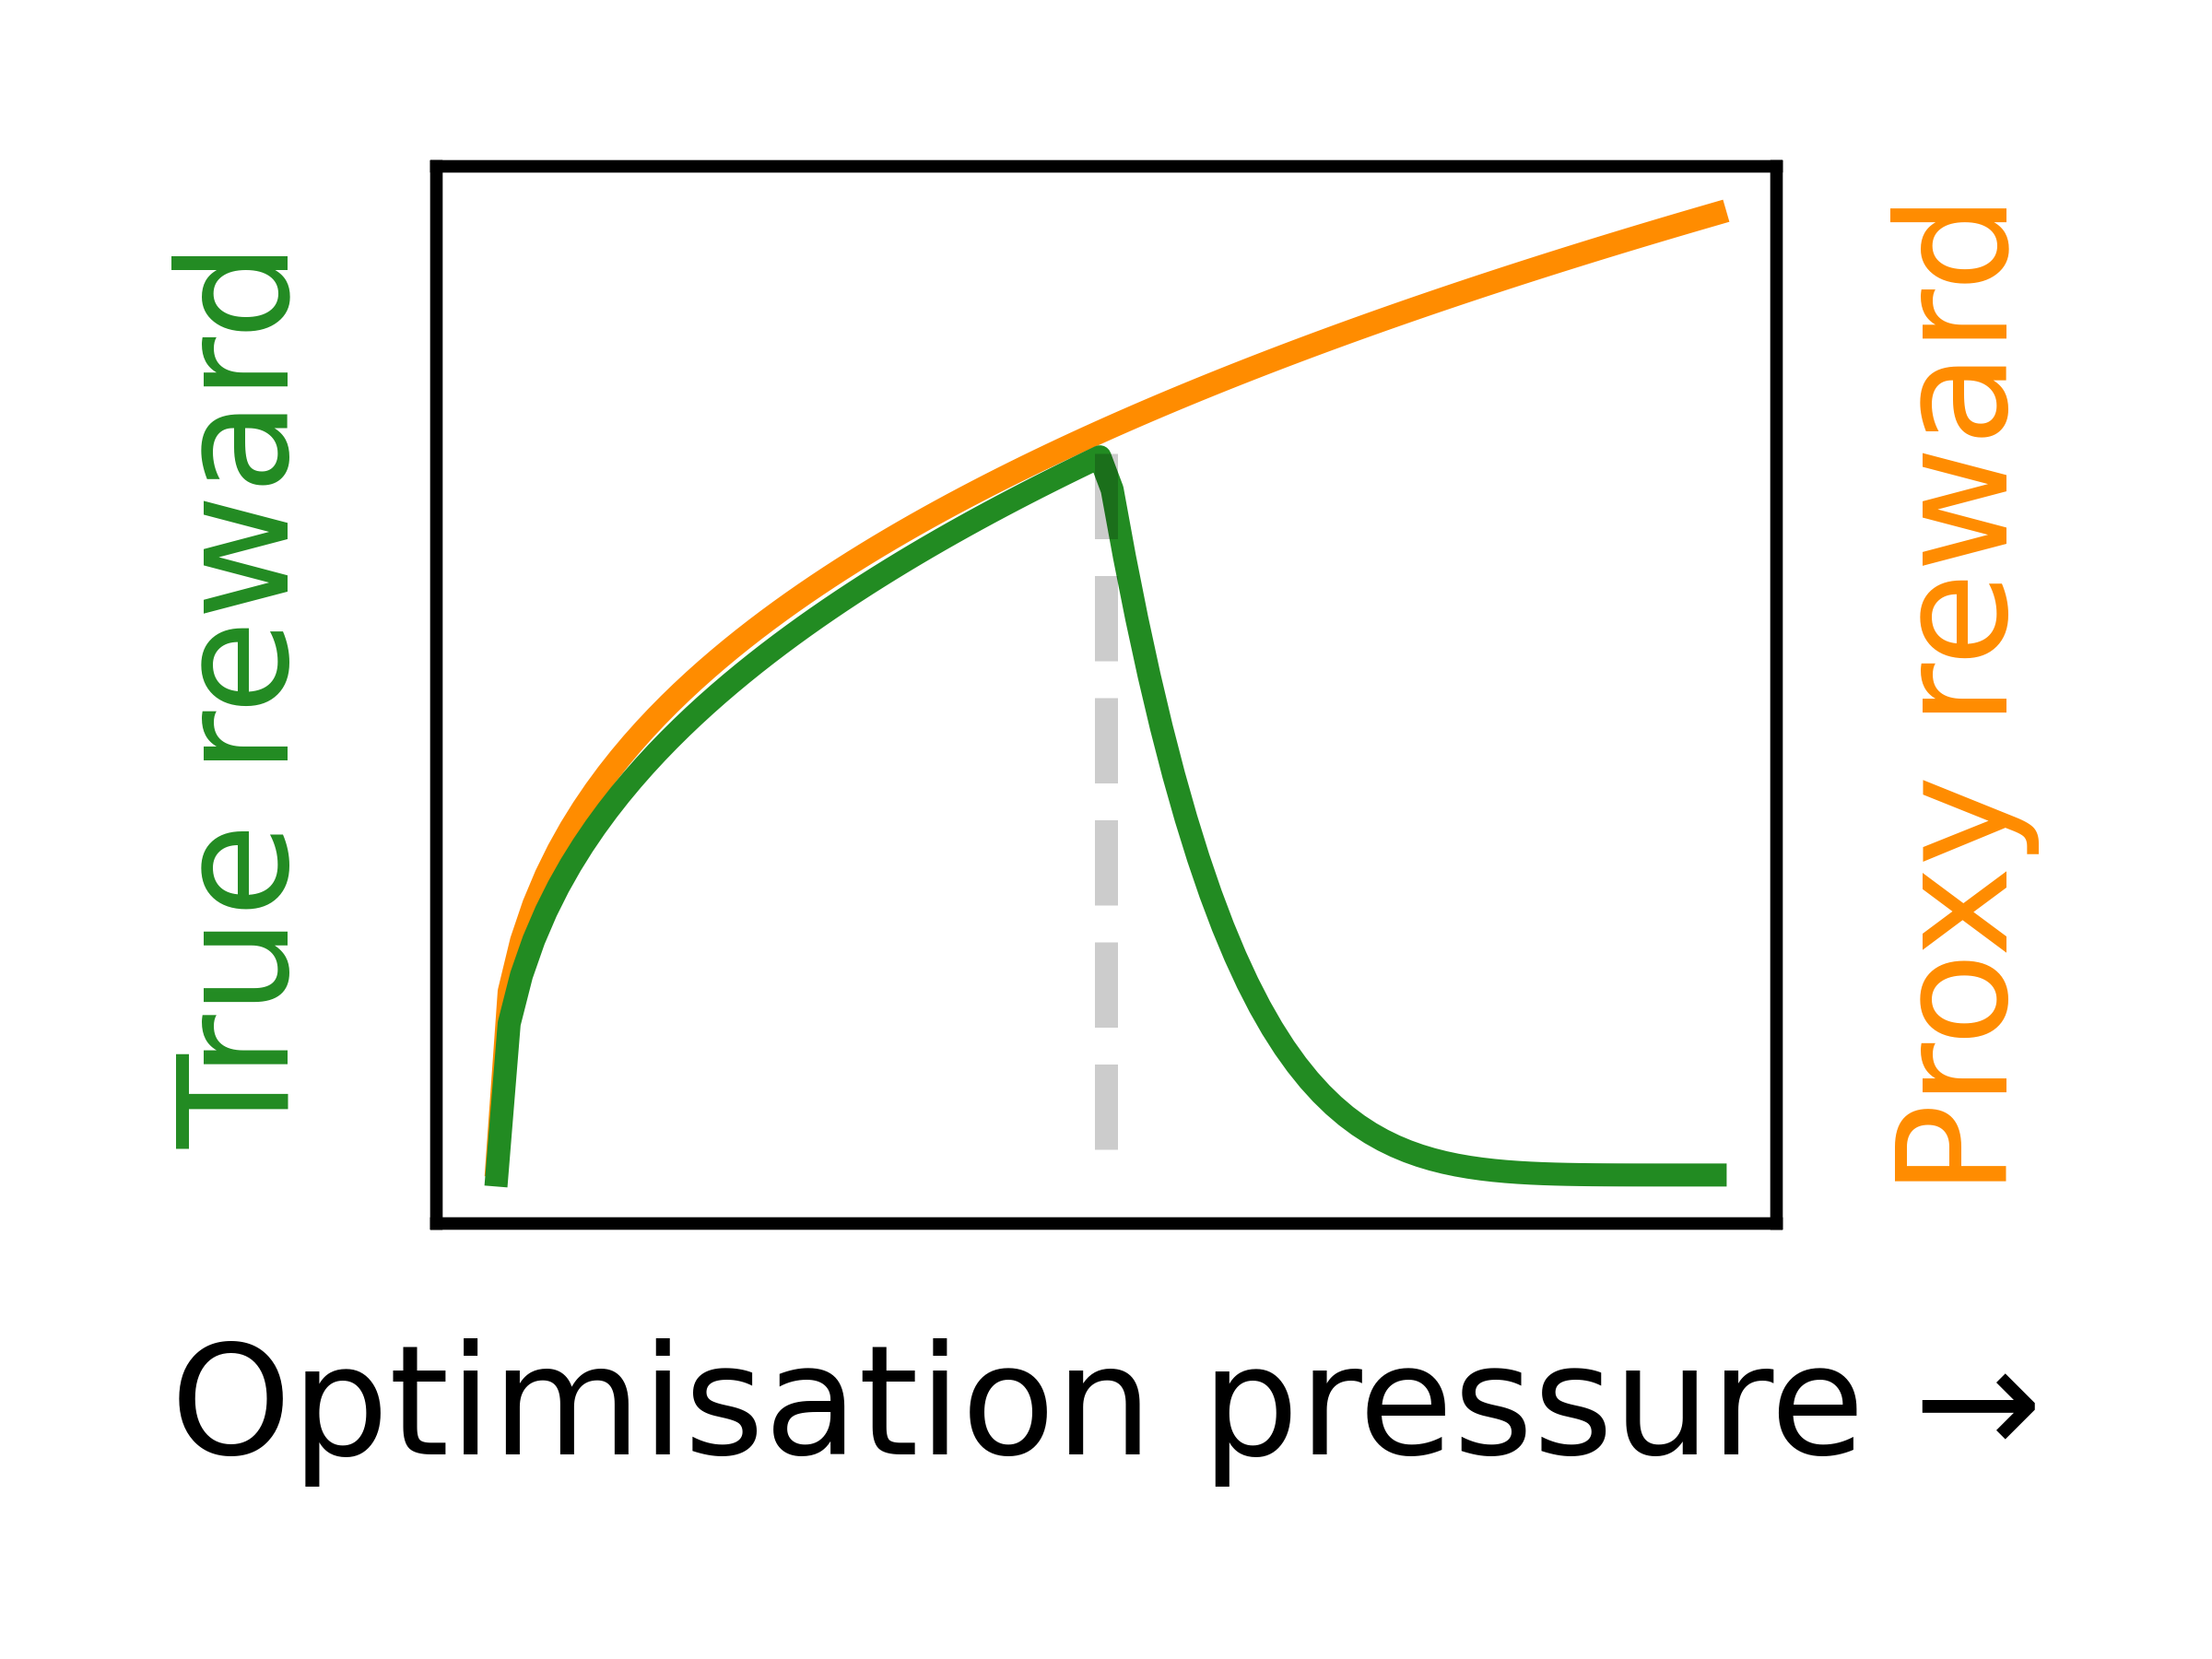
\includegraphics[width=\linewidth]{other_figures/cartoon.png}
    \vspace{-6mm}  % 10
    \caption{A cartoon of Goodharting.}
    \label{fig:goodhart_cartoon}
    \vspace{-7mm}  % 10
\end{wrapfigure}

In this paper, we present several novel contributions. 
First, we show that \enquote{Goodharting} occurs with high probability for a wide range of environments and pairs of true and proxy reward functions. Next, we provide a mechanistic explanation of \emph{why} Goodhart's law emerges in RL. 
We use this to derive two new policy optimisation methods and show that they \emph{provably} avoid Goodharting. 
Finally, we evaluate these methods empirically.
We thus contribute towards building a better understanding of the dynamics of optimising towards imperfect proxy reward functions, and show that these insights may be used to design new algorithms.